% II-4-7 Fork-Join Sorting Application — БД2 Final Report
% Compile: xelatex II-4-7_Final_Report.tex   (2 удаа; Overleaf дээр Compiler = XeLaTeX)
\documentclass[11pt,a4paper]{article}

\usepackage{fontspec}
% Кирилл (Ө, Ү) дэмждэг фонт. macOS/Windows: Times New Roman + Menlo/Consolas.
% Overleaf дээр: \setmainfont{DejaVu Serif} ба \setmonofont{DejaVu Sans Mono} болгож солино.
\setmainfont{Times New Roman}
\setmonofont{Menlo}[Scale=0.85]

\usepackage[margin=2.2cm]{geometry}
\usepackage{graphicx}
\usepackage{booktabs}
\usepackage{tabularx}
\usepackage{array}
\usepackage{longtable}
\usepackage{xcolor}
\usepackage{caption}
\usepackage{float}
\usepackage{enumitem}
\usepackage{tikz}
\usetikzlibrary{arrows.meta,positioning,fit,calc}
\usepackage{pgfplots}
\pgfplotsset{compat=1.17}
\usepackage[hidelinks]{hyperref}

\graphicspath{{../screenshots/bd2/}}
\captionsetup{font=small,labelfont=bf}
\renewcommand{\figurename}{Зураг}
\renewcommand{\tablename}{Хүснэгт}
\renewcommand{\refname}{Ашигласан материал}
\newcommand{\todo}[1]{\textcolor{red}{[#1]}}
\newcolumntype{Y}{>{\raggedright\arraybackslash}X}
\setlength{\parskip}{4pt}
\setlist{itemsep=1pt,topsep=3pt}

\begin{document}

% ------------------------------------------------------------------ Нүүр
\begin{titlepage}
\centering
{\large ШИНЖЛЭХ УХААН ТЕХНОЛОГИЙН ИХ СУРГУУЛЬ\par}
{Мэдээлэл, холбооны технологийн сургууль\par}
\vspace{3cm}
{\Huge\bfseries FINAL REPORT\par}
\vspace{0.6cm}
{\Large Fork-Join Sorting Application\par}
\vspace{0.4cm}
{F.CSM302 Үйлдлийн систем · Бие даалт 2\par}
{2026--2027 оны хичээлийн жилийн намар\par}
\vfill
\begin{tabular}{ll}
Хуваарилалтын код: & \textbf{II-4-7} \\
Хичээл заасан багш: & Г. Ганбат /F.CS10/ \\
Шүүмжилсэн баг: & IV-2-10 \\
Repository: & \url{https://github.com/NamiIwbr/fork-join-sorting} \\
Хувилбар: & \texttt{v2.0.0} \todo{commit hash} \\[6pt]
Гишүүд: & Б. Намуун /B241930008/ \\
 & О. Түвшин /B241940139/ \\
 & Э. Тайванбаяр /B242270068/ \\
 & П. Мөнхжаргал /B221960805/ \\
 & Ц. Мөнхжин /B232270034/ \\
 & Д. Дашбалбар /B251940502/ \\
\end{tabular}
\vspace{2cm}

Улаанбаатар хот, 2026 он
\end{titlepage}

% ------------------------------------------------------------------ Хураангуй
\section*{Хураангуй}

БД1-д Merge Sort ба Quick Sort-ийг Java-ийн \texttt{ForkJoinPool}, \texttt{RecursiveAction} ашиглан зэрэгцээ
эрэмбэлж, recursion tree дээр алхамчлан харуулсан. Шүүмжлэгч баг (IV-2-10) ба багшийн санал нэг гол дутагдлыг
онцолсон: програм алгоритмын дарааллыг сайн тайлбарлаж байсан ч \emph{хэзээ, хаана fork ба join хийгдэж, аль
thread юу гүйцэтгэж байгааг} харуулдаггүй байв. Үйлдлийн системийн хичээлд thread бол үндсэн агуулга юм.

БД2-т дараах гол сайжруулалтыг хийсэн:
\begin{itemize}
  \item Task бүрийн worker thread, fork/join цэг, хугацааг бодитоор бүртгэж (\texttt{ExecutionLog}), \textbf{thread
        timeline} ба үйл явдлын бүртгэл дээр work stealing-ийг харуулсан.
  \item Recursion tree дээр \texttt{fork()}/\texttt{compute()}/\texttt{join()} ирмэг, FORK/JOIN алхам, зангилаа бүрт
        түүнийг гүйцэтгэсэн thread-ийн тэмдэг нэмсэн.
  \item Эрэмбэлэлтийг JavaFX UI thread-ээс background thread руу шилжүүлсэн.
  \item \texttt{mvn test} ба CI, хоосон массив, буруу параметр, thread-ийн шинэ тест нэмж, нийт шалгалтыг
        9\,111-ээс 11\,946 болгосон (бүгд амжилттай).
\end{itemize}
Хэмжилтээр 1 сая элемент дээр 8 worker 1 worker-оос 3.8--4.4 дахин хурдан, мөн BD1-ээс 2.3--3.7 дахин хурдан
болсон нь нотлогдсон.

% ------------------------------------------------------------------ 1
\section{Төслийн тойм}

Сурах бичгийн 4-р бүлгийн \emph{Fork-Join Sorting Application} төсөл нь эрэмбэлэлтийг divide-and-conquer
хэлбэрээр Java Fork-Join framework дээр хэрэгжүүлэхийг шаарддаг~[1]. Fork-Join загварт эцэг task ажлаа дэд
task-уудад хувааж (\emph{fork}), тэдгээрийг зэрэгцээ гүйцэтгүүлж, дуусахыг хүлээн (\emph{join}) үр дүнг
нэгтгэнэ~[1,~2]. Хүснэгт~\ref{tab:req}-д номын шаардлага ба БД2-ийн хэрэгжилтийг харьцуулав.

\begin{table}[H]
\centering
\caption{Сурах бичгийн шаардлага ба хэрэгжилт}
\label{tab:req}
\begin{tabularx}{\textwidth}{@{}lY@{}}
\toprule
Шаардлага & Хэрэгжилт \\
\midrule
Хоёр алгоритм & \texttt{MergeSortTask}, \texttt{QuickSortTask} (generic, \texttt{T extends Comparable<T>}) \\
\texttt{RecursiveAction} & Хоёр класс удамшуулсан, \texttt{ForkJoinPool.invoke()}-оор эхэлнэ \\
Хуваалт & Merge: ойролцоо тэнцүү хоёр хагас; Quick: median-of-three pivot, гурван хэсгийн хуваалт \\
Threshold & Хэсгийн урт $\le$ threshold үед insertion sort \\
Fork / join & \texttt{second.fork(); first.compute(); second.join();} (БД2) \\
UI дүрслэл & Recursion tree + бодит thread timeline (БД2) \\
\bottomrule
\end{tabularx}
\end{table}

% ------------------------------------------------------------------ 2
\section{Эцсийн архитектур}

Зураг~\ref{fig:arch}-д БД2-ийн бүрэлдэхүүн, өгөгдлийн урсгалыг үзүүлэв. Ногоон хүрээтэй нь БД2-т шинээр
нэмэгдсэн, шар хүрээтэй нь өөрчлөгдсөн бүрэлдэхүүн. Хамгийн чухал өөрчлөлт нь UI thread ба тооцооллын thread-ийг
салгаж, бодит гүйцэтгэлийн бүртгэлийг дүрслэлтэй холбосон явдал юм.

\begin{figure}[H]
\centering
\begin{tikzpicture}[
  box/.style={draw,rounded corners=3pt,minimum width=3.2cm,minimum height=0.85cm,align=center,font=\small},
  new/.style={box,draw=green!50!black,line width=1.2pt,fill=green!6},
  chg/.style={box,draw=orange!80!black,line width=1.2pt,fill=orange!6},
  arr/.style={-{Stealth[length=2.2mm]},thick},
  node distance=0.6cm and 1.0cm]
  \node[chg] (main) {Main\\(JavaFX UI thread)};
  \node[new,right=of main] (parser) {InputParser\\оролт шалгах};
  \node[chg,below=of main] (task) {javafx Task\\\texttt{sort-runner} thread};
  \node[new,right=of task] (runner) {SortRunner\\pool W1..Wn};
  \node[chg,below=of runner] (fj) {Merge/QuickSortTask\\fork · compute · join};
  \node[new,right=of fj] (log) {ExecutionLog\\START/FORK/JOIN/END};
  \node[chg,below=of fj] (node) {SortNode мод\\thread, хугацаа};
  \node[box,below=of task] (trace) {SortTrace\\алхмын тайлбар};
  \node[chg,below=1.4cm of trace] (tree) {TreeCanvas\\fork/join ирмэг, T·W};
  \node[new,right=2.2cm of tree] (tl) {ThreadTimeline\\worker lane, event log};
  \draw[arr] (main) -- (parser);
  \draw[arr] (main) -- node[left,font=\scriptsize]{Эрэмбэлэх} (task);
  \draw[arr] (task) -- (runner);
  \draw[arr] (runner) -- node[right,font=\scriptsize]{invoke} (fj);
  \draw[arr] (fj) -- (log);
  \draw[arr] (fj) -- (node);
  \draw[arr] (task) -- node[left,font=\scriptsize]{$n\le32$} (trace);
  \draw[arr] (trace) -- node[left,font=\scriptsize]{onSucceeded (UI)} (tree);
  \draw[arr] (node) |- (tl);
  \draw[arr,dashed] (tree) -- node[above,font=\scriptsize]{сонгосон task} (tl);
\end{tikzpicture}
\caption{БД2-ийн архитектур (ногоон = шинэ, шар = өөрчлөгдсөн)}
\label{fig:arch}
\end{figure}

Бүрэлдэхүүн тус бүрийн үүрэг ба БД1-ээс ялгаатай нь Хүснэгт~\ref{tab:comp}-д байна.

\begin{table}[H]
\centering
\caption{Өөрчлөгдсөн ба шинэ бүрэлдэхүүн}
\label{tab:comp}
\begin{tabularx}{\textwidth}{@{}lY@{}}
\toprule
Файл & БД2-ийн өөрчлөлт \\
\midrule
\texttt{MergeSortTask}, \texttt{QuickSortTask} & \texttt{invokeAll}-ийг тодорхой fork/compute/join-оор сольж, цэг бүрийг бүртгэнэ. Quick Sort-д ганц дэд хэсэг үлдвэл fork хийхгүй. \\
\texttt{ExecutionLog} (шинэ) & Олон thread-ээс \texttt{ConcurrentLinkedQueue}-д үйл явдал бичнэ; worker бүрийн task, ажилласан хугацаа, steal тоолно. \\
\texttt{SortRunner} (шинэ) & W1..Wn нэртэй worker-тэй \texttt{ForkJoinPool} үүсгэж, task-уудад preorder дугаар (T1..) олгоно. GUI ба тест хоёулаа ашиглана. \\
\texttt{SortNode} & Thread, эхэлсэн/fork/join хүлээсэн/join дууссан/дууссан хугацаа, fork эсэх, steal эсэх. \\
\texttt{ThreadTimeline} (шинэ) & Worker бүрийн мөр, task-ийн хэсгүүд, steal ба join сум, үйл явдлын бүртгэл. \\
\texttt{TreeCanvas}, \texttt{SortTrace} & FORK/COMPUTE/JOIN алхам, ирмэгийн төлөв, T·W тэмдэг. \\
\texttt{Main}, \texttt{InputParser} & Background Task, worker тоо ба leaf саатлын тохиргоо, оролтын шалгалтыг тусгаарласан. \\
\bottomrule
\end{tabularx}
\end{table}

\paragraph{Синхрончлол.} \texttt{SortNode}-ийн талбаруудыг зөвхөн тухайн task-ийг гүйцэтгэж буй thread бичдэг.
Эцэг task эдгээрийг \texttt{join()}-ийн дараа, UI нь \texttt{pool.invoke()} дууссаны дараа уншдаг. Энэ хоёр үйлдэл
happens-before холбоо үүсгэдэг тул нэмэлт lock шаардлагагүй~[6]. Олон thread зэрэг бичдэг цорын ганц бүтэц болох
үйл явдлын жагсаалтад lock-free \texttt{ConcurrentLinkedQueue} ашигласан.

% ------------------------------------------------------------------ 3
\section{Туршилт ба дүрслэл}

Хэрэглэгч дараах параметрүүдийг өөрчилж, дэлгэцийн хоёр хэсгээс үр дүнг ажиглана:
\begin{itemize}
  \item \textbf{Өөрчлөх:} өгөгдөл, threshold, алгоритм, worker-ийн тоо (Auto/1/2/4/8), leaf саатал (0--500 ms).
  \item \textbf{Recursion tree (дээд):} FORK алхамд эцгээс \texttt{compute()} (цэнхэр) ба \texttt{fork()} (тасархай
        нил ягаан) ирмэг гарна. JOIN алхамд ногоон \texttt{↑ join()} болно. Зангилаа бүрийн \texttt{T3·W2} тэмдэг нь
        task-ийг бодитоор гүйцэтгэсэн worker-ийг заана.
  \item \textbf{Thread timeline (доод):} мөр бүр нэг worker. Хайрцаг нь task-ийн өөрийн ажил, саарал зурвас нь
        \texttt{join()} хүлээлт, нил ягаан сум нь өөр worker-ийн хулгайлсан fork, ногоон сум нь join-оор буцалт.
\end{itemize}

Модны анимаци нь дарааллыг ойлгуулах тайлбар, харин timeline нь бодит \texttt{System.nanoTime} хэмжилт гэдгийг UI-д
тодорхой бичсэн (шүүмж A2). Хоёрыг холбохын тулд модны одоогийн алхам солигдоход харгалзах task timeline дээр
тодордог. Зураг~\ref{fig:fork}-д анхны тохиргоо (8 тоо, threshold 2, саатал 20 ms)-ны FORK алхмыг үзүүлэв. Timeline
дээр дөрвөн leaf (T3, T4, T6, T7) дөрвөн өөр worker дээр зэрэг ажиллаж байгаа нь харагдана.

\begin{figure}[H]
\centering
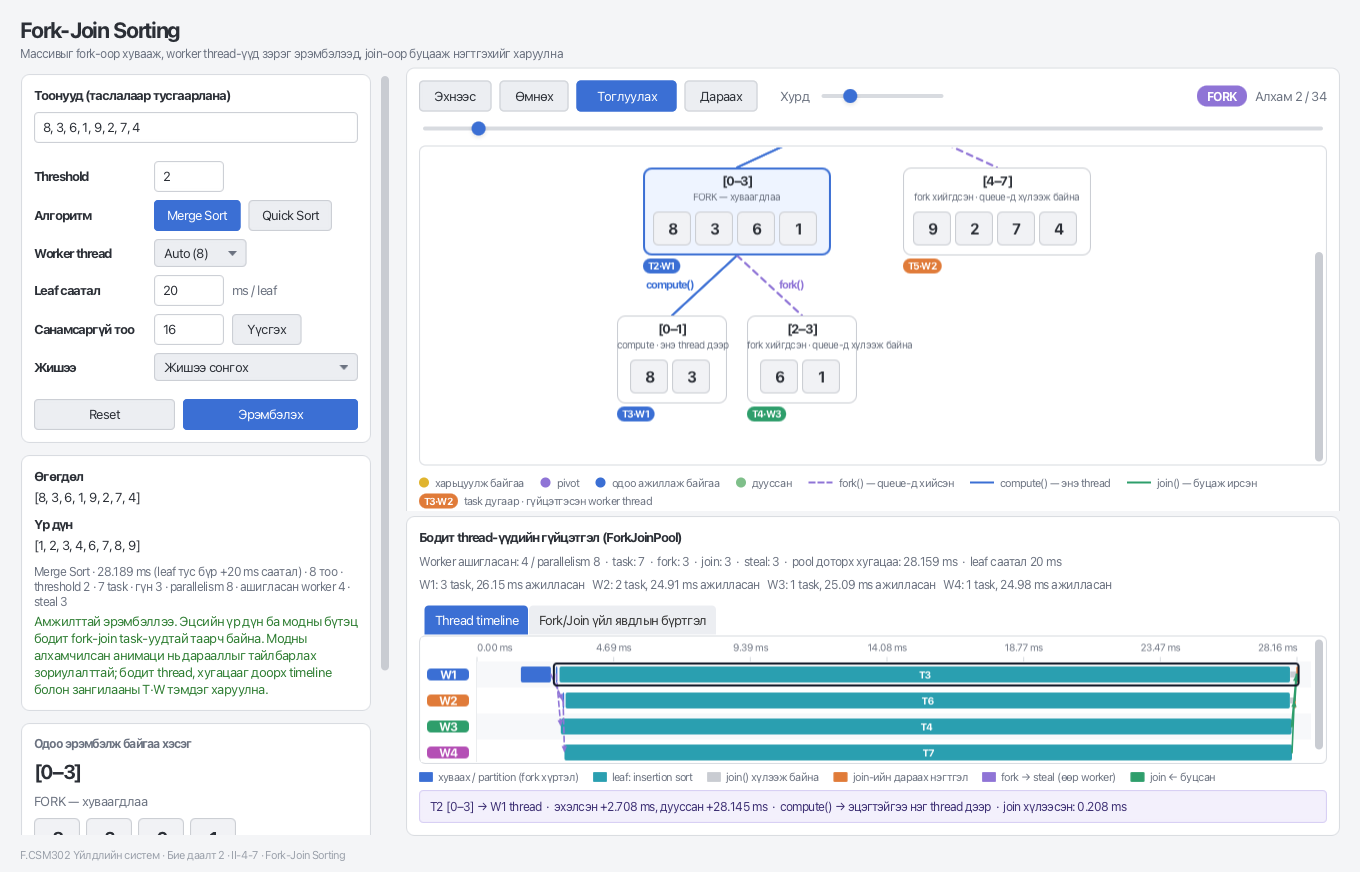
\includegraphics[width=\textwidth]{01_fork_step_merge.png}
\caption{Merge Sort-ийн FORK алхам ба 4 worker-ийн бодит timeline}
\label{fig:fork}
\end{figure}

% ------------------------------------------------------------------ 4
\section{Reviewer Responses}

Албан ёсны шүүмж (\texttt{Review\_II\_4\_7.pdf}) ба багшийн саналыг нэгтгэж, Peer Review удирдамжийн түвшингээр
ангилсан. Хүснэгт~\ref{tab:resp}-д шүүмж бүрийн шийдвэр, өөрчлөлт ба нотолгоог үзүүлэв. Зөвшөөрөөгүй санал
байхгүй, гишүүдийн оролцооны саналыг хэсэгчлэн хүлээн авсан.

{\small
\begin{longtable}{@{}p{0.4cm}p{4.1cm}p{1.5cm}p{1.6cm}p{6.8cm}@{}}
\caption{Reviewer Comments and Responses}\label{tab:resp}\\
\toprule
№ & Шүүмж & Priority & Шийдвэр & Өөрчлөлт ба нотолгоо \\
\midrule
\endfirsthead
\toprule
№ & Шүүмж & Priority & Шийдвэр & Өөрчлөлт ба нотолгоо \\
\midrule
\endhead
1 & Багш: хэзээ, хаана fork/join хийгдэхийг харуулах; thread бол үндсэн агуулга & Major & Зөвшөөрсөн &
  Тодорхой fork/compute/join, \texttt{ExecutionLog}, \texttt{ThreadTimeline}, ирмэг ба T·W тэмдэг, worker тоо. Зураг~\ref{fig:fork}--\ref{fig:steal}; тест N5--N7. \\
2 & A1: \texttt{pool.invoke()} UI thread дээр хүлээнэ & Major & Зөвшөөрсөн &
  \texttt{javafx.concurrent.Task}, \texttt{sort-runner} thread; ажиллах үед оролт идэвхгүй, давхар эхлүүлэхгүй. 5000 элемент дээр UI хариу өгсөөр. \\
3 & A2: «мод бодит fork-join-той яг таарна» мэдэгдэл хэт ерөнхий; task/thread ID, эхлэх/дуусах бүртгэх & Minor & Зөвшөөрсөн &
  Мэдэгдлийг засаж, анимаци = тайлбар гэж тодруулсан. Үйл явдлын бүртгэл (Зураг~\ref{fig:log}). Тест N5. \\
4 & A3: Manual-ийн \texttt{javac} команд гурван мөрөнд тасарсан & Minor & Зөвшөөрсөн &
  Үндсэн команд \texttt{mvn clean test}; нэг мөрийн macOS/Linux ба Windows хувилбар; README = Manual. \\
5 & A4: \texttt{mvn test}, CI, Quick threshold=0, хоосон массив (T06) & Suggestion & Зөвшөөрсөн &
  JUnit 5 + Surefire, GitHub Actions; N1, N2, N4 тест. \\
6 & A4: гишүүдийн үүрэг, commit холбоос & Minor & Хэсэгчлэн &
  Хүснэгт~\ref{tab:members}-д бодит оролцоог бичсэн; commit түүх нэг account-оос тул бусад ажлыг тайланд тодорхойлсон. \\
7 & A5: \texttt{target/} repository-д & Minor & Зөвшөөрсөн &
  \texttt{git rm --cached -r target}, \texttt{.gitignore}. \\
8 & Өөрсдөө олсон: task бүр дэд массивыг текст болгодог & Major & Зөвшөөрсөн &
  Зөвхөн $\le 32$ элементэд. 1 сая элемент дээр 2.3--3.7× хурдан (Хүснэгт~\ref{tab:before}). \\
\bottomrule
\end{longtable}
}

% ------------------------------------------------------------------ 5
\section{Дахин туршилт}

Өөрчлөлтийн дараа BD1-ийн бүх тестийг өөрчлөлтгүйгээр (regression) дахин ажиллуулж, шинэ тест нэмсэн. Хүснэгт
\ref{tab:regr}-д засварын өмнөх ба дараах үр дүнг харьцуулав. BD1-ийн 9\,111 шалгалт хэвээр амжилттай байгаа нь
үндсэн функц хадгалагдсаныг харуулна.

\begin{table}[H]
\centering
\caption{Regression ба шинэ тест (\texttt{mvn clean test})}
\label{tab:regr}
\begin{tabularx}{\textwidth}{@{}Yll@{}}
\toprule
Тест & БД1 (831c55c) & БД2 \\
\midrule
BD1 regression (номын жишээ, захын тохиолдол, 1500 санамсаргүй, 10\,000, String) & 9111 / 0 & 9111 / 0 \\
N1 хоосон массив (T06) & --- & 6 / 0 \\
N2 буруу параметр (Quick threshold 0, $-1$, null, муж) & --- & 8 / 0 \\
N3 Int-ийн хязгаар, шүүмжлэгчийн \texttt{3,-1,3,0} & --- & PASS \\
N4 GUI оролт (\texttt{InputParser}) & --- & 18 / 0 \\
N5 fork/join бүртгэл: 200 массив × 2 алгоритм, 1--4 worker & --- & PASS \\
N6 parallelism 1: нэг thread, steal 0 & --- & PASS \\
N7 4 worker, 40 ms leaf: зэрэг ажилласан (15 давталт) & --- & PASS \\
\midrule
\textbf{Нийт (passed / failed)} & \textbf{9111 / 0} & \textbf{11946 / 0} \\
\bottomrule
\end{tabularx}
\end{table}

N5 тест бодит гүйцэтгэлийн бүртгэл үнэн зөв эсэхийг шалгана. Үүнд дараах нөхцөлүүд орно:
START ба END үйл явдлын тоо task-ийн тоотой тэнцүү, FORK ба JOIN тоо тэнцүү, хүүхэд task эцгийнхээ fork-оос хойш
эхэлж join-оос өмнө дуусна, \texttt{compute()}-оор ажилласан хүүхэд эцэгтэйгээ нэг thread дээр байна, тайлбарын
trace-ийн FORK/JOIN алхмын тоо бодит fork/join-той тэнцүү.

% ------------------------------------------------------------------ 6
\section{Эцсийн үр дүн}

\subsection{Thread-ийн ажиглалт}

Worker-ийн тоог өөрчлөхөд гүйцэтгэл хэрхэн өөрчлөгдөхийг Зураг~\ref{fig:one}-д үзүүлэв. Ижил өгөгдөл
(8 тоо, threshold 2, саатал 20 ms) Worker = 1 үед бүх 7 task W1 дээр дараалан ажиллаж 98.5 ms зарцуулсан. Auto
(8) үед 4 worker ашиглагдаж, 3 steal болж 28.2 ms болсон (Зураг~\ref{fig:fork}).

\begin{figure}[H]
\centering
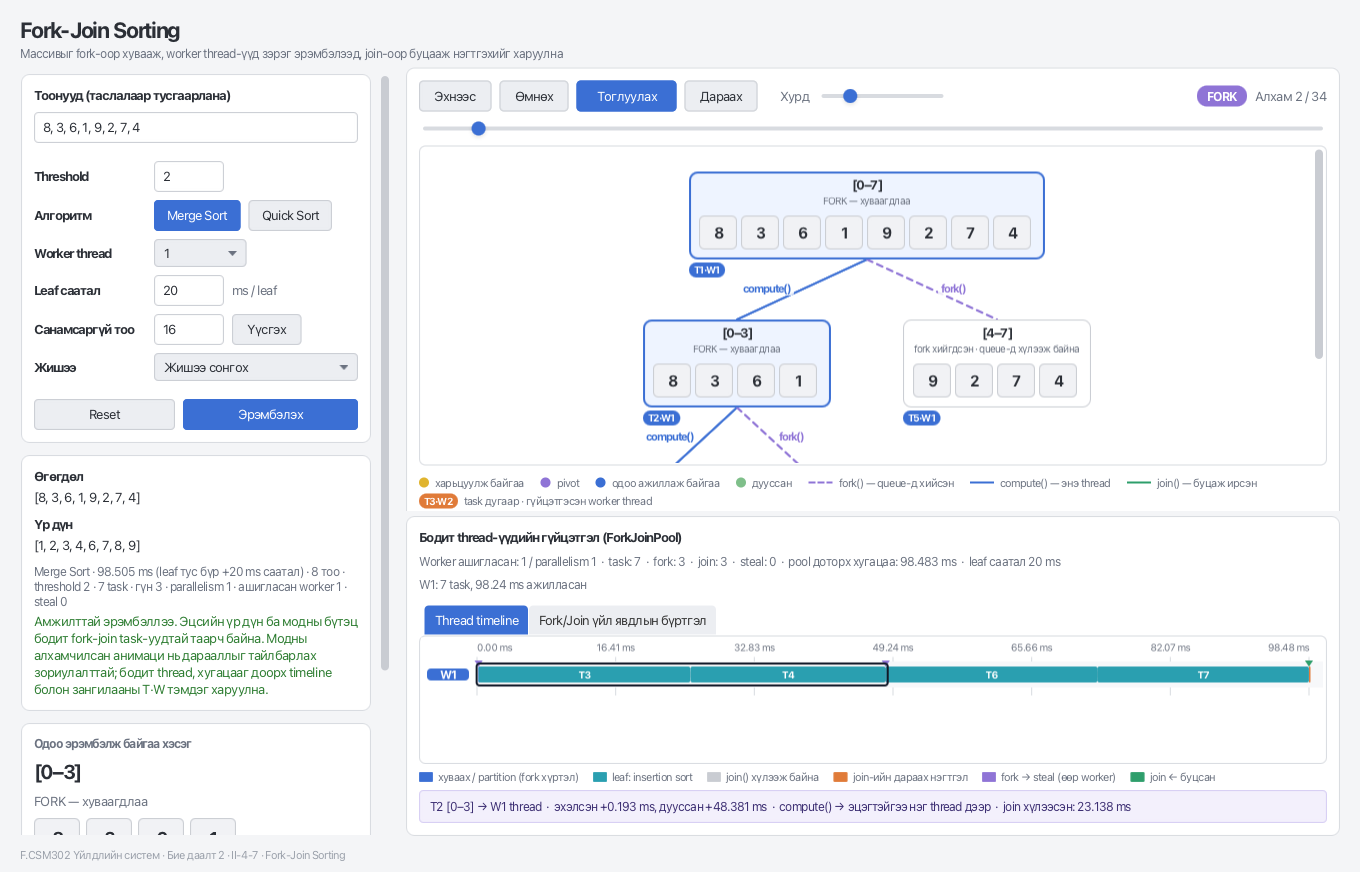
\includegraphics[width=0.92\textwidth]{06_one_worker.png}
\caption{Worker = 1: бүх task нэг thread дээр дараалан (steal 0)}
\label{fig:one}
\end{figure}

Зураг~\ref{fig:steal}-д Quick Sort-ийн work stealing-ийг харуулав. W1 fork хийсэн T3-г W2, W2 fork хийсэн T6-г W3
хулгайлж ажиллуулсан. Энэ хооронд W1, W2 нь \texttt{join()} дээр хүлээж байна (саарал зурвас). Энэ нь Fork-Join
pool-ийн work-stealing scheduler~[2,~3]-ийн ажиллагааг бодит өгөгдлөөр харуулж байна.

\begin{figure}[H]
\centering
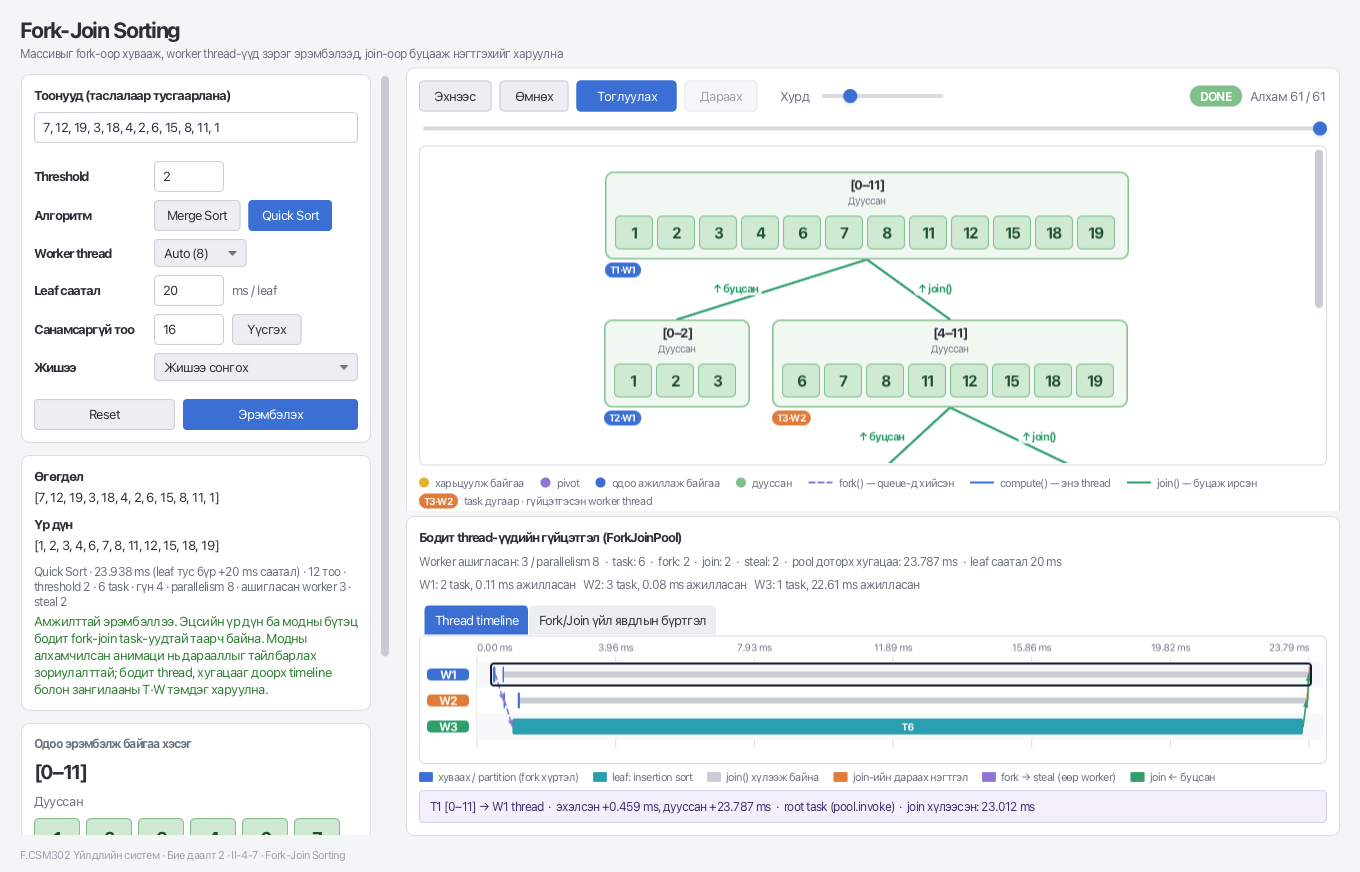
\includegraphics[width=0.92\textwidth]{05_quick_work_stealing.png}
\caption{Quick Sort: fork хийгдсэн task-уудыг өөр worker хулгайлсан (work stealing)}
\label{fig:steal}
\end{figure}

Зураг~\ref{fig:log}-д task бүрийн START, FORK, COMPUTE, JOIN, END үйл явдлыг thread ба хугацаатай нь харуулсан
бүртгэлийг үзүүлэв (шүүмж A2).

\begin{figure}[H]
\centering
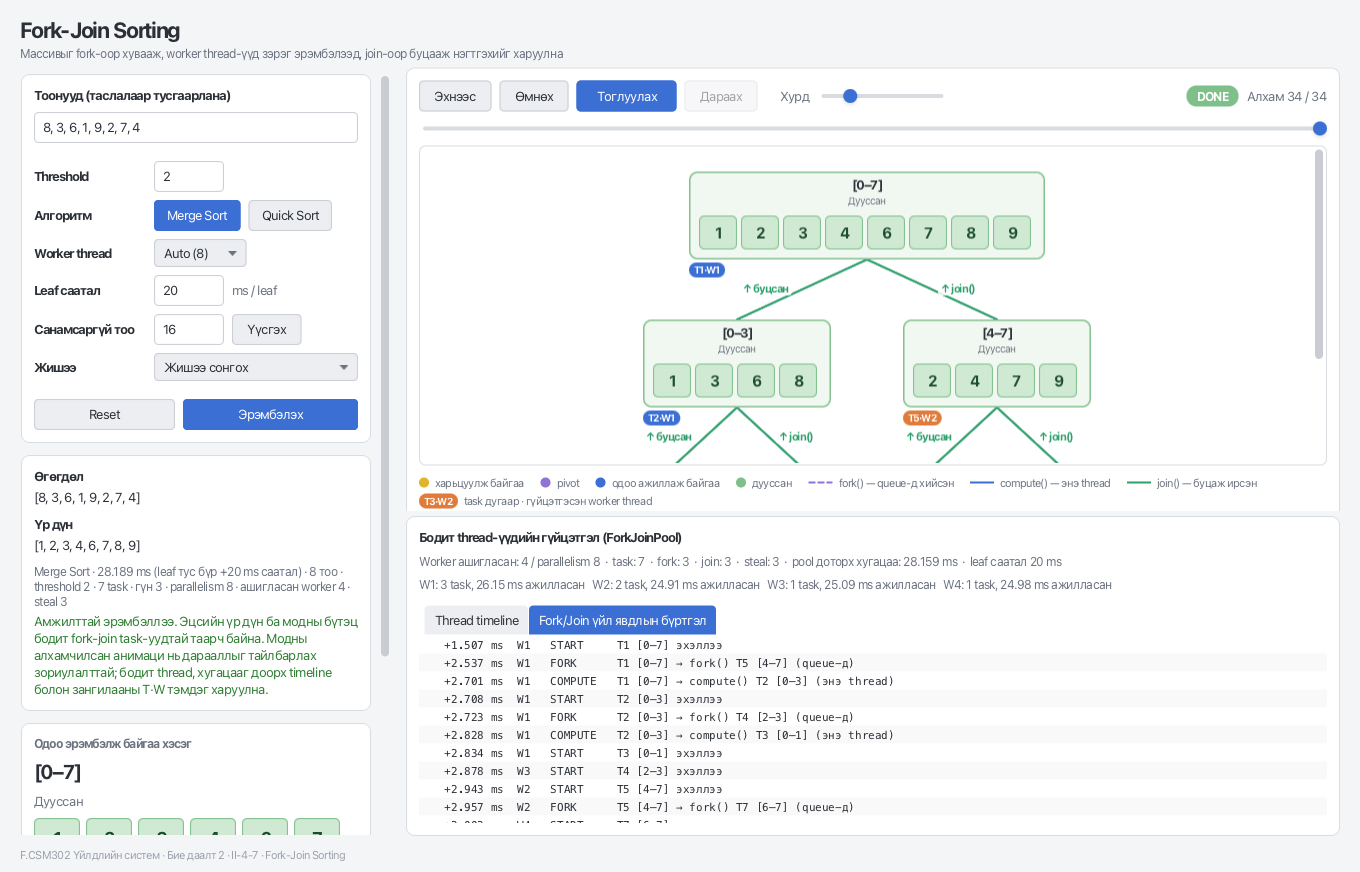
\includegraphics[width=0.92\textwidth]{04_event_log.png}
\caption{Fork/Join үйл явдлын бүртгэл}
\label{fig:log}
\end{figure}

\subsection{Гүйцэтгэлийн хэмжилт}

Хэмжилтийг Apple M1 (4 performance + 4 efficiency цөм), Java 23.0.1 дээр 1\,000\,000 санамсаргүй \texttt{Integer}
(seed 2026)-ээр хийсэн. Тохиргоо бүрийг 3 удаа халааж, 5 удаа хэмжиж median авсан (\texttt{tests/Benchmark.java}).
Зураг~\ref{fig:speedup} ба Хүснэгт~\ref{tab:speed}-д worker-ийн тоо ба хурдсалтыг үзүүлэв.

\begin{figure}[H]
\centering
\begin{tikzpicture}
\begin{axis}[width=0.62\textwidth,height=5.2cm,xlabel={Worker thread},ylabel={Хурдсалт $T(1)/T(p)$},
  xtick={1,2,4,8},xmode=log,log basis x=2,log ticks with fixed point,ymin=0,ymax=8.5,grid=major,
  legend pos=north west,legend style={font=\small}]
\addplot[mark=*,thick,blue] coordinates {(1,1.00) (2,1.90) (4,3.34) (8,4.35)};
\addplot[mark=square*,thick,orange] coordinates {(1,1.00) (2,1.95) (4,3.13) (8,3.77)};
\addplot[dashed,gray] coordinates {(1,1) (2,2) (4,4) (8,8)};
\legend{Merge Sort,Quick Sort,Шугаман (идеал)}
\end{axis}
\end{tikzpicture}
\caption{Worker-ийн тоо ба хурдсалт (threshold 1000, $n=10^6$)}
\label{fig:speedup}
\end{figure}

\begin{table}[H]
\centering
\caption{Worker-ийн тоо ба хугацаа (threshold 1000, median ms)}
\label{tab:speed}
\begin{tabular}{@{}lrrrr@{}}
\toprule
Алгоритм & 1 worker & 2 worker & 4 worker & 8 worker \\
\midrule
Merge Sort & 816.9 & 430.7 & 244.6 & 187.7 \\
Quick Sort & 565.8 & 290.2 & 180.7 & 150.0 \\
Steal (Merge / Quick) & 0 / 0 & 2 / 6 & 11 / 16 & 71 / 107 \\
\bottomrule
\end{tabular}
\end{table}

Хурдсалт шугаман биш байгаа нь Amdahl-ийн хуулиар~[4] тайлбарлагдана: root-ийн сүүлийн merge болон эхний partition
нь нэг thread дээр дараалан явагддаг. Мөн M1-ийн 8 цөмийн 4 нь бага чадалтай. Threshold-ийн нөлөөг
Хүснэгт~\ref{tab:th}-д үзүүлэв.

\begin{table}[H]
\centering
\caption{Threshold-ийн нөлөө (8 worker, median ms)}
\label{tab:th}
\begin{tabular}{@{}lrrrrrr@{}}
\toprule
Threshold & 16 & 64 & 256 & 1024 & 4096 & 16384 \\
\midrule
Merge Sort & 211.1 & \textbf{56.8} & 72.0 & 191.8 & 1358.1 & 7694.1 \\
Quick Sort & 370.7 & \textbf{104.5} & 119.6 & 189.8 & 856.9 & 4506.9 \\
\bottomrule
\end{tabular}
\end{table}

Threshold бага үед task үүсгэх, fork/join-ийн зардал давамгайлдаг. Их үед leaf бүрийн insertion sort $O(t^2)$
болж~[5] огцом удааширдаг. Энэ машин дээр оновчтой утга ойролцоогоор 64 байна.

Эцэст нь BD1 ба BD2-ийн кодыг ижил нөхцөлд (8 worker, тус бүр шинэ JVM дээр 3 удаа) харьцуулсныг
Хүснэгт~\ref{tab:before}-д үзүүлэв.

\begin{table}[H]
\centering
\caption{BD1 ба BD2-ийн харьцуулалт ($n=10^6$, 8 worker, 3 ажиллуулалтын median)}
\label{tab:before}
\begin{tabular}{@{}llrrr@{}}
\toprule
Алгоритм & Threshold & BD1, ms & BD2, ms & Хурдсалт \\
\midrule
Merge Sort & 1000 & 604.7 & 241.6 & 2.5× \\
Quick Sort & 1000 & 695.9 & 187.5 & 3.7× \\
Merge Sort & 16 & 712.6 & 305.7 & 2.3× \\
Quick Sort & 16 & 800.5 & 309.9 & 2.6× \\
\bottomrule
\end{tabular}
\end{table}

% ------------------------------------------------------------------ 7
\section{Хязгаарлалт}

Програмд дараах хязгаарлалт, анхаарах зүйлс үлдсэн:
\begin{itemize}
  \item Recursion tree-ийн алхамчилсан дүрслэл $\le 32$ элементэд л ажиллана. Timeline бүх хэмжээнд ажиллана.
  \item Модны анимаци нь нэг thread-ээр тооцоолсон тайлбарын дараалал. Бодит зэрэгцээ дарааллыг timeline тусад нь
        харуулна.
  \item Жижиг өгөгдөлд task-ууд микросекундэд дуусдаг тул leaf саатал (\texttt{Thread.sleep}) нэмж байж
        зэрэгцээ ажиллагаа нүдэнд харагдана. Энэ саатал нийт хугацаанд орно.
  \item Хугацааны хэмжилт нь OS-ийн thread scheduling, JVM-ийн JIT ба GC-ээс хамаарч ажиллуулалт бүрт ±15--30\%
        хэлбэлздэг.
  \item Шалгасан орчин: macOS 14 (Apple M1), JDK 23.0.1; CI: Ubuntu, Temurin JDK 23.
\end{itemize}

% ------------------------------------------------------------------ 8
\section{Дүгнэлт}

БД2-т шүүмжийн бүх Major асуудлыг шийдэж, программыг «алгоритмын тайлбар»-аас «thread-ийн ажиллагааг харуулах»
хэрэгсэл болгосон. Хэрэглэгч одоо fork хийгдсэн task-ийг аль worker хулгайлж, join дээр хэн хэр удаан хүлээснийг
бодит хугацаагаар харж чадна. Мөн worker-ийн тоог өөрчилж хурдсалтыг шууд ажиглана.

Төслөөс суралцсан гол зүйлс:
\begin{itemize}
  \item Fork-Join-ийн үр ашиг нь ажлын хэмжээ ба fork-ийн зардлын харьцаанаас шууд хамаардаг. Threshold-ийн
        оновчтой утга хэмжилтээр олдоно.
  \item Work stealing нь join дээр хүлээж буй thread-ийг сул зогсоолгүй, өөр task-ийг хулгайлж гүйцэтгүүлдэг.
  \item UI thread дээр хүнд тооцоолол хийхгүй байх, мөн thread хоорондын happens-before холбоог зөв ашиглах нь
        чухал.
  \item Шүүмж, хэмжилт нь бидний анзаараагүй гүйцэтгэлийн алдааг (2.3--3.7× удаашрал) илрүүлэхэд тусалсан.
\end{itemize}

% ------------------------------------------------------------------ Гишүүд
\section*{Хавсралт. Гишүүдийн ажил хариуцлага}

Хүснэгт~\ref{tab:members}-д гишүүн бүрийн БД2 дахь бодит оролцоог бичнэ (шүүмж A4).

\begin{table}[H]
\centering
\caption{Гишүүдийн ажил хариуцлага (БД2)}
\label{tab:members}
\begin{tabularx}{\textwidth}{@{}lYl@{}}
\toprule
Гишүүн & Хариуцсан ажил & Commit / файл \\
\midrule
Б. Намуун & \todo{бөглөнө} & \todo{} \\
О. Түвшин & \todo{бөглөнө} & \todo{} \\
Э. Тайванбаяр & \todo{бөглөнө} & \todo{} \\
П. Мөнхжаргал & \todo{бөглөнө} & \todo{} \\
Ц. Мөнхжин & \todo{бөглөнө} & \todo{} \\
Д. Дашбалбар & \todo{бөглөнө} & \todo{} \\
\bottomrule
\end{tabularx}
\end{table}

AI-ийн хэрэглээ: BD2-ийн кодын сайжруулалт, тест, баримт бичгийн ноорогт Claude (Anthropic)-ийг туслах хэрэгсэл
болгон ашигласан. Бүх өөрчлөлтийг баг шалгаж, тестээр баталгаажуулсан.

% ------------------------------------------------------------------ Ном зүй
\begin{thebibliography}{9}
\bibitem{osc} A. Silberschatz, P. B. Galvin, G. Gagne, \emph{Operating System Concepts}, 10th ed. Hoboken, NJ:
  Wiley, 2018, ch.~4 (Threads \& Concurrency).
\bibitem{lea} D. Lea, ``A Java fork/join framework,'' in \emph{Proc. ACM 2000 Conf. on Java Grande}, San Francisco,
  CA, 2000, pp.~36--43.
\bibitem{bl} R. D. Blumofe, C. E. Leiserson, ``Scheduling multithreaded computations by work stealing,''
  \emph{Journal of the ACM}, vol.~46, no.~5, pp.~720--748, 1999.
\bibitem{amdahl} G. M. Amdahl, ``Validity of the single processor approach to achieving large scale computing
  capabilities,'' in \emph{Proc. AFIPS Spring Joint Computer Conf.}, 1967, pp.~483--485.
\bibitem{clrs} T. H. Cormen, C. E. Leiserson, R. L. Rivest, C. Stein, \emph{Introduction to Algorithms}, 3rd ed.
  Cambridge, MA: MIT Press, 2009.
\bibitem{jcip} B. Goetz et al., \emph{Java Concurrency in Practice}. Boston, MA: Addison-Wesley, 2006.
\end{thebibliography}

\end{document}
